\begin{document}
\chapter{Results}
\section{Error and convergence from simulated data} \label{simDataError}
Data is produced through simulations with different kinds and magnitudes of noise. Two kinds of results are presented:
\begin{itemize}
\item The convergence of a simulation from an erroneous initial position, erroneous initial receiver clock bias and both an erroneous initial position and receiver clock bias.
\item The trend of error in final convergence value for an increasing noise of different kinds.
\end{itemize} 
The noise types introduced are as follows:
\begin{itemize}
\item Noise free
\item Receiver clock bias
\item Satellite position random noise
\item Measurement white noise
\end{itemize}

\subsection{Convergence of estimate for noise free measurements with different initial error}
The results of simulations of the convergence of the state estimates $\boldsymbol \theta$ as a function of the number of iterations is shown in figure \ref{fig:sim_est_pos_conv}. When adding an error to the initial estimate is tested, the initial estimate ${\boldsymbol \theta}_0$ will be equal to the true state ${\boldsymbol \theta}$ plus a random noise in all three components the position of increasing magnitude of 10 to $10^7$ m. 
\par
The simulations were found to converge with an initial state error in the position of magnitude up to $10^7$m in all directions. MATLAB uses 16 digits of precision by default, meaning that the error is expected to converge to that precision, these results are assumed to be due to observations being in the range of approximately 2$\sim$3$\cdot 10^7$ m making an observation registered with eight digits of precision. When adding noise to the satellite position, a random noise is added to the satellite position of increasing magnitude from 1 to $10^3$ m. When adding a random noise is tested, a random noise is added to the observations of increasing magnitude from 1 to $10^3$ m. 
\par 
\begin{figure}[!h]
    \centering % <-- added
\begin{subfigure}{0.49\textwidth}
  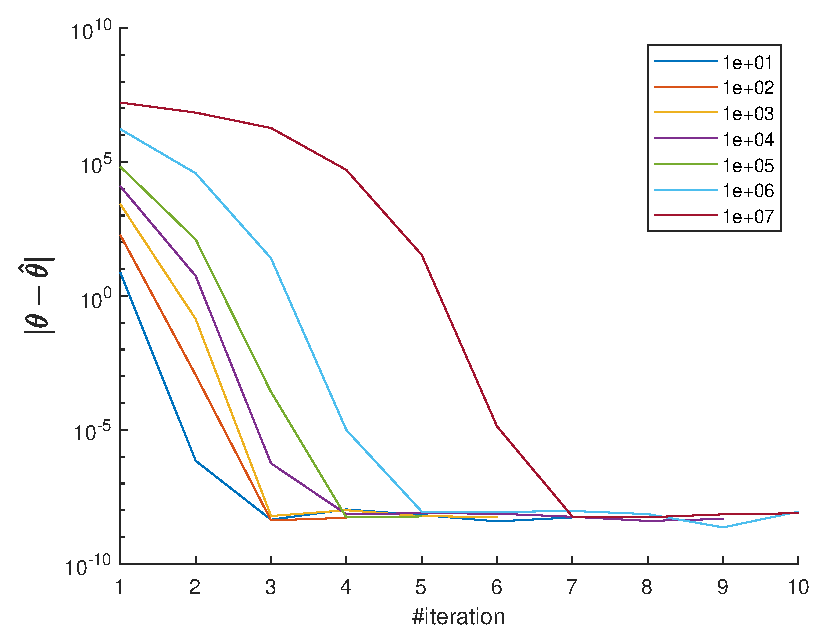
\includegraphics[width=\linewidth]{Results/SimulationEstPos/noiseFreeConv}
\end{subfigure}\hfil % <-- added
\medskip
\begin{subfigure}{0.49\textwidth}
  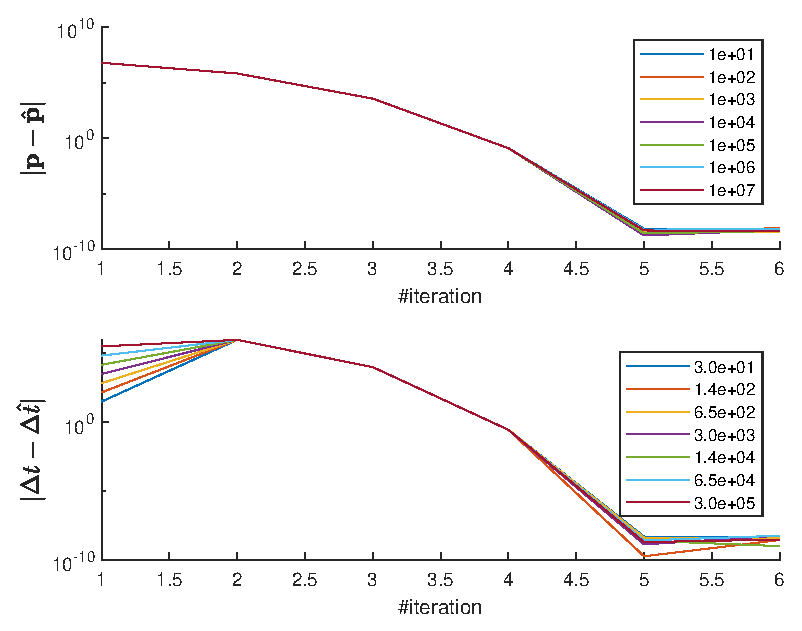
\includegraphics[width=\linewidth]{Results/SimulationEstPos/clockBConv}
\end{subfigure}\hfil % <-- added
\medskip
\begin{subfigure}{0.49\textwidth}
  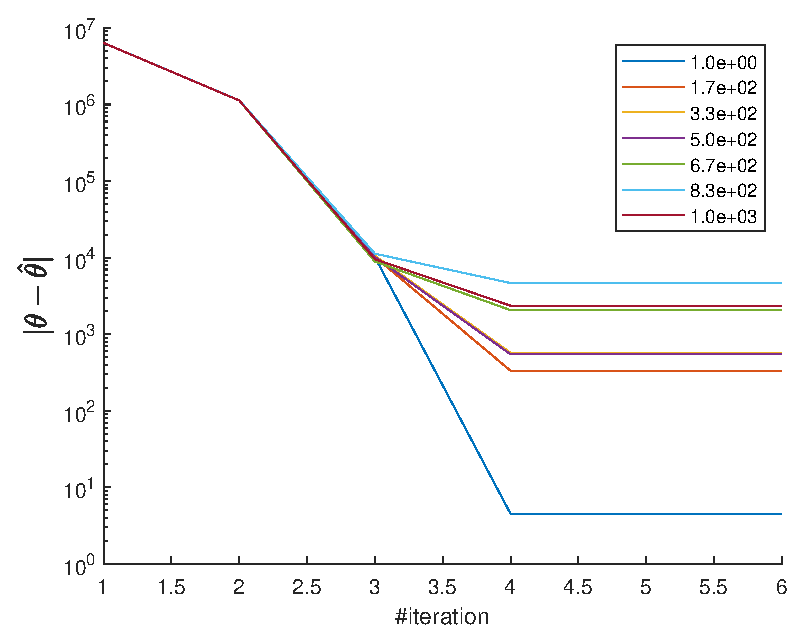
\includegraphics[width=\linewidth]{Results/SimulationEstPos/satPosConv}  
\end{subfigure}
\medskip
\begin{subfigure}{0.49\textwidth}
  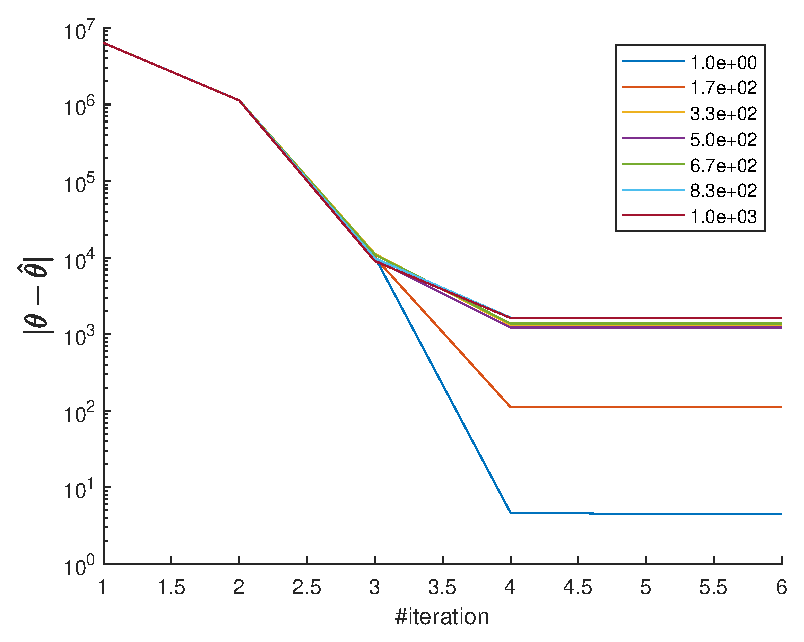
\includegraphics[width=\linewidth]{Results/SimulationEstPos/GaussianConv}
\end{subfigure}
\caption{Simulation results with different input noise. From top left to bottom right: a)Noise free, b) Clock bias, c) Satellite position, f) Gaussian noise. In figure a), different error in starting positions is tested. The horizontal axis shows the number of iterations and vertical axis shows the norm of the error between true and estimated states $|{\boldsymbol \theta}-\hat{{\boldsymbol \theta}}|$.} 
\label{fig:sim_est_pos_conv}
\end{figure}
In figure \ref{fig:mixedConv} the convergence of an erroneous initial state is presented. For any magnitude of initial error in all parameters between $10^{-10}$ to $10^5$ m the parameters converge to the correct value within the interruption threshold of the estimator function.

\begin{figure}[htb]
    \centering % <-- added
  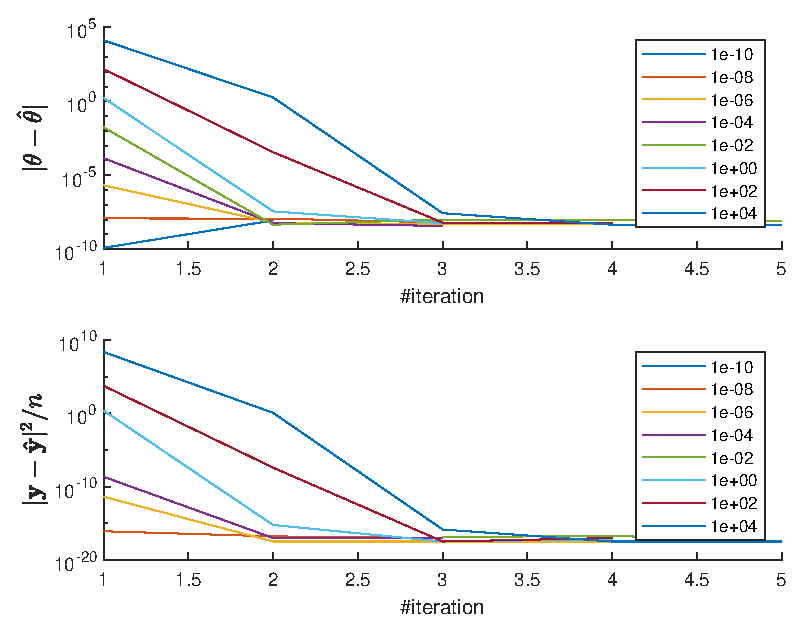
\includegraphics[width=0.8\linewidth]{Results/SimulationEstPos/mixedNoiseConv}
\caption{\label{fig:mixedConv} The plots show the convergence behaviour with noise free estimates and an initial random error in both position and clock bias of increasing magnitude. Upper: error in $|{\boldsymbol \theta}-\hat{{\boldsymbol \theta}}|$ per iteration. Lower: mean square error in estimated observation}
\end{figure}	

\subsection{Final estimate for added measurement noise of different magnitudes}
The results to the error in the terminal estimate of receiver states when adding noise of increasing magnitude is simulated. The result is presented in figure \ref{fig:sim_est_pos}. In the upper graph, three types of errors are shown: $|\bf p-\hat{p}|$ where $\bf p$ is the true position and $\bf \hat{p}$ indicates a least-squares estimate, similarly $|{\boldsymbol \theta}-\hat{{\boldsymbol \theta}}|$, where the mean square error is given by the sum $\frac{1}{n}\sum (y-\hat{y}))^2$ where a simulated observation is produced as that given in equation (\ref{ObsRange}), and thus $\hat{y}$ is the predicted measurement given the calculated satellite's position and estimated state of the receiver from equation (\ref{hModel}). \\
\begin{figure}[!h]
    \centering % <-- added
\begin{subfigure}{0.49\textwidth}
  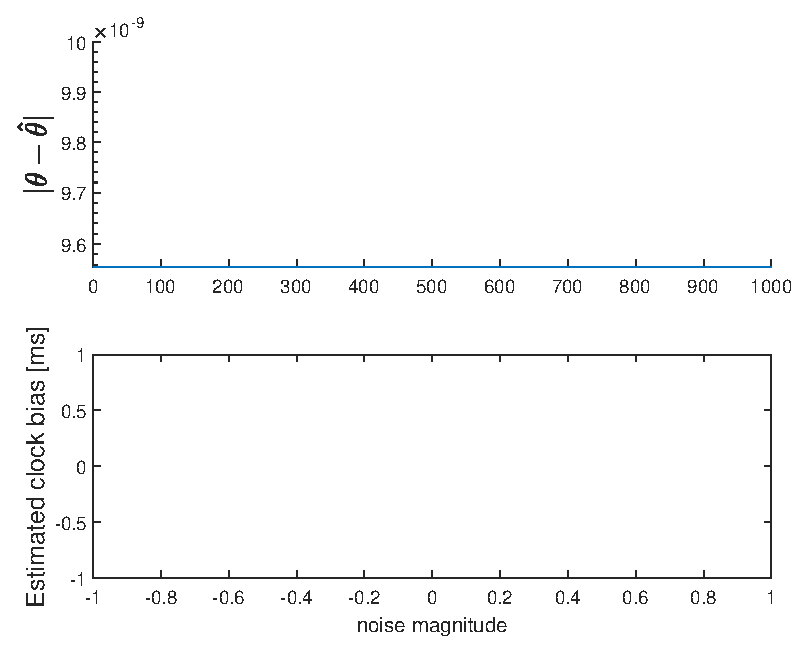
\includegraphics[width=\linewidth]{Results/SimulationEstPos/noiseFree}
\end{subfigure}\hfil % <-- added
\medskip
\begin{subfigure}{0.49\textwidth}
  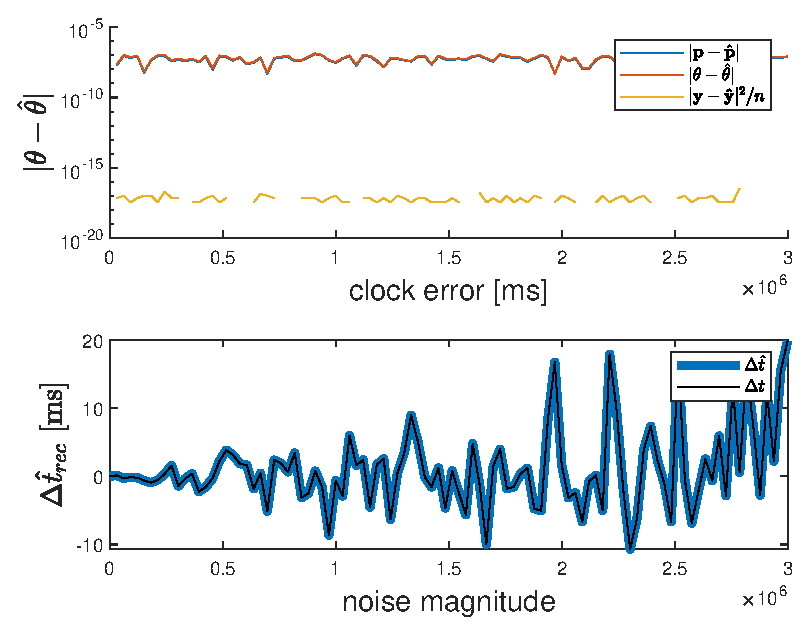
\includegraphics[width=\linewidth]{Results/SimulationEstPos/clockB}
\end{subfigure}\hfil % <-- added
\medskip
\begin{subfigure}{0.49\textwidth}
  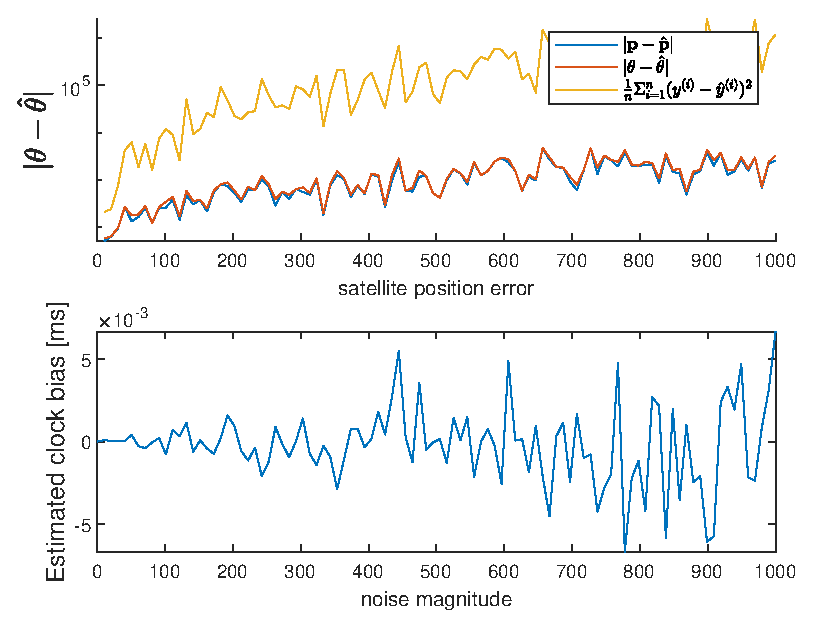
\includegraphics[width=\linewidth]{Results/SimulationEstPos/satPos}  
\end{subfigure}
\medskip
\begin{subfigure}{0.49\textwidth}
  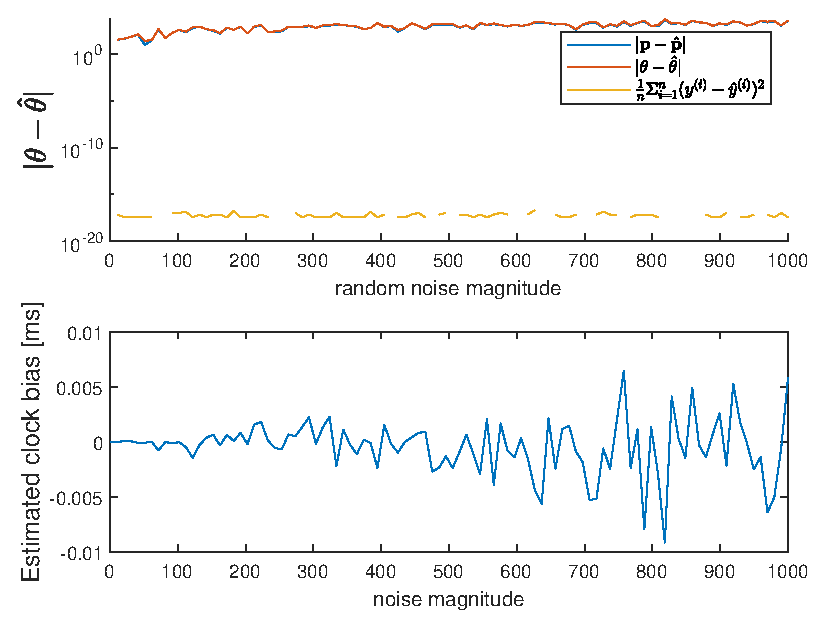
\includegraphics[width=\linewidth]{Results/SimulationEstPos/Gaussian}
\end{subfigure}
\caption{Simulation results with different input noise. From top left to bottom right: a)Noise free, b) Clock bias, c) Satellite position, d) Gaussian noise. Note that a) converges to 0 for all iterations. The upper figure in each pair shows the norm of the error in position: $|\bf p-\hat{p}|$, position+clock bias $|\bf \theta-\hat{\theta}|$ and expected observation mean square error $\frac{1}{n}\sum(y-\hat{y})^2$ as function of noise magnitude and the bottom figure the calculated clock bias as function of noise magnitude.}
\label{fig:sim_est_pos}
\end{figure}
\par
The simulations show that for an error consisting only of receiver clock bias, the effect on the positioning is negligible, as $|\textbf{p}-\hat{\textbf{p}}|$ lies steadily around $10^{-10}$. For other types of added noise, the error appear to grow at the same rate as that of the noise source.

\section{Calculating satellite position}\label{satelliteTrajectory}
The satellite positions are calculated in accordance with the method described in section \ref{chap:ephPositioning}. The position is presented in two forms, the position in the sky over time in a polar chart without any corresponding time stamp, as well as 1D graphs of  elevation with regards to the position of the receiver given by the onboard electronics. For measurements taken on April 11, 2019, starting at 12:25:28 (UTC), the skyplot of the calculated satellite positions are shown in figure \ref{fig:skyplot}, next to that available at online source\footnote{link to reconstruct plot: 
\url{https://www.gnssplanning.com/\#/embedded?satellites=1,2,3,5,6,7,8,9,10,11,12,13,14,15,16,17,18,19,20,21,22,23,24,25,26,27,28,29,30,31,32&satSystems=GPS&restoreSats=0&target=settings&cutoffDeg=0&durationHours=6&utcTime=2019-04-11T12:00:00&hgt=10&lonDeg=18.0687918056&latDeg=59.3481576111}
}
\begin{figure}
\begin{minipage}{0.49\textwidth}
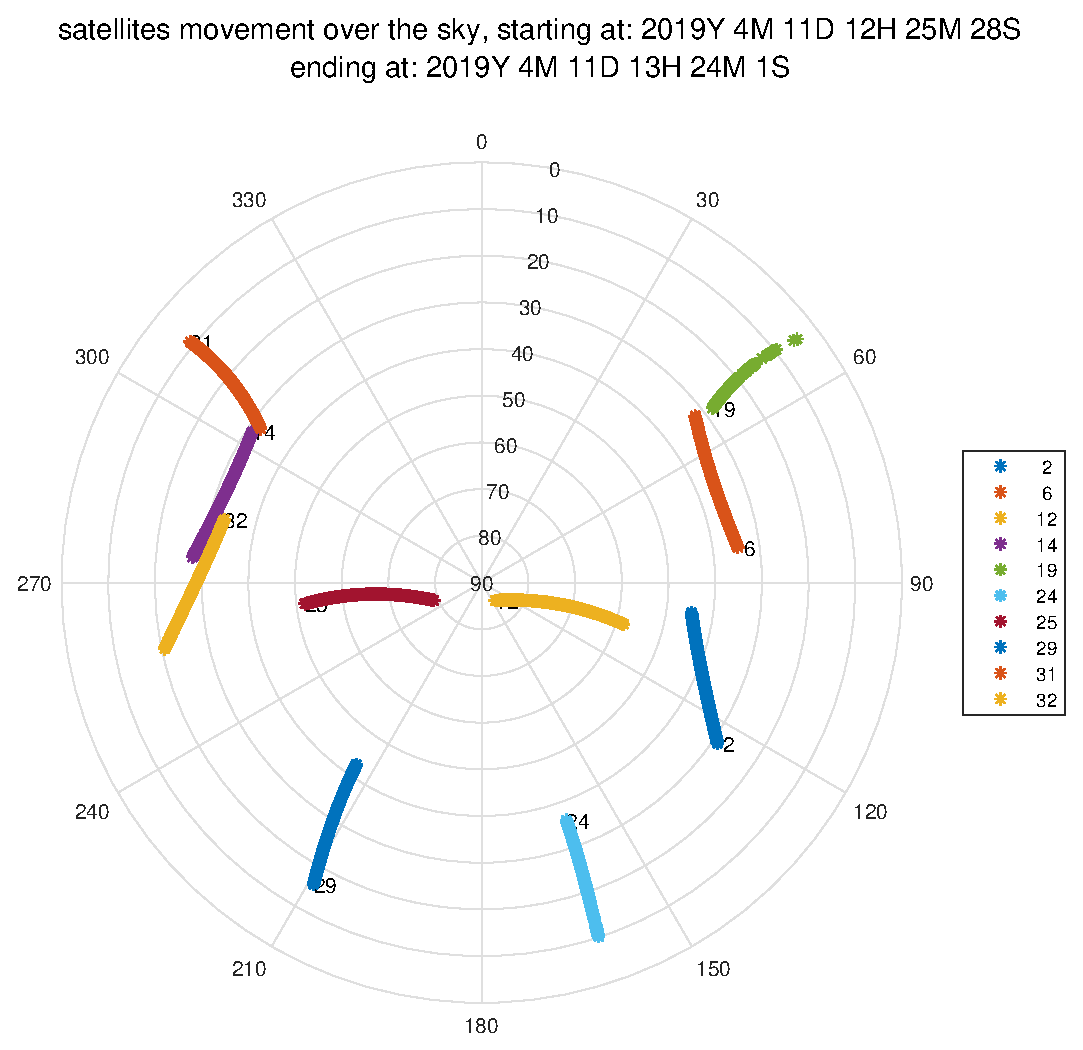
\includegraphics[width=\textwidth]{Results/satsInSky.eps}
\caption{\label{fig:skyplot} GPS Satellite's movement in the sky for the duration of the measurement, only showing when they are observed by the receiver.}
\end{minipage}
\begin{minipage}{0.49\textwidth}
\vspace{3 mm}
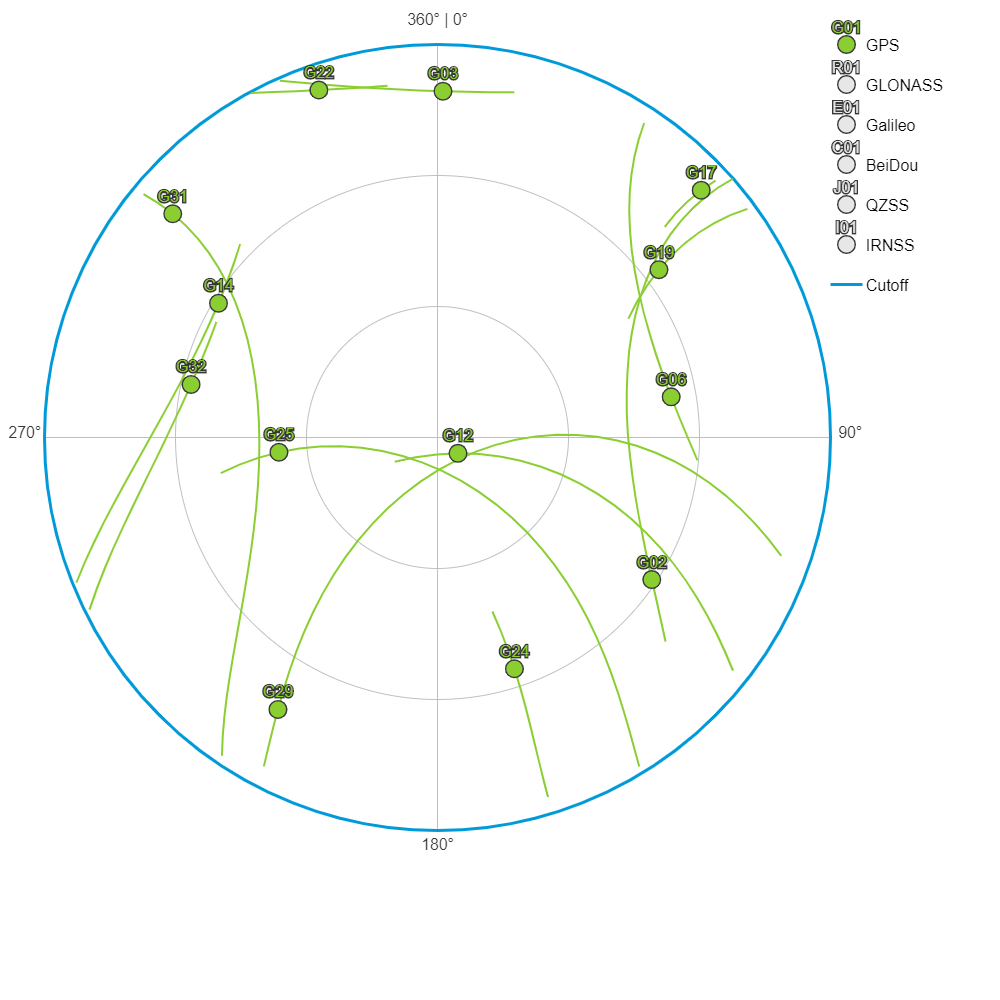
\includegraphics[width=\textwidth]{Results/skyplot190411-1230}
\caption{\label{fig:skyplotGNSSPLANNING} Skyplot for all visible GPS-satellites at UTC 2019-04-11, 12:30 Stockholm, Sweden from \url{www.gnssplanning.com}. Trajectories indicated without direction}
\end{minipage}
\end{figure}
The elevation, azimuth and distance calculations for the GPS satellites over the same time interval as indicated in figure \ref{fig:skyplot} is shown in figure \ref{fig:el6H}. The corresponding elevation over time for the satellites in figure (\ref{fig:skyplotGNSSPLANNING}) is shown in figure \ref{fig:elGNSSPlanning}. Note that the time interval is larger in figure \ref{fig:elGNSSPlanning} than that of \ref{fig:el6H} due to only actually sampled satellite ephemeris data is used and satellites only being visible for a short time period. 
\par 
A coarse evaluation indicates that the solutions are equal. The precision with which the satellite positions can be evaluated is however quite low with regards to a fine positioning solution.
\begin{figure}[!h]
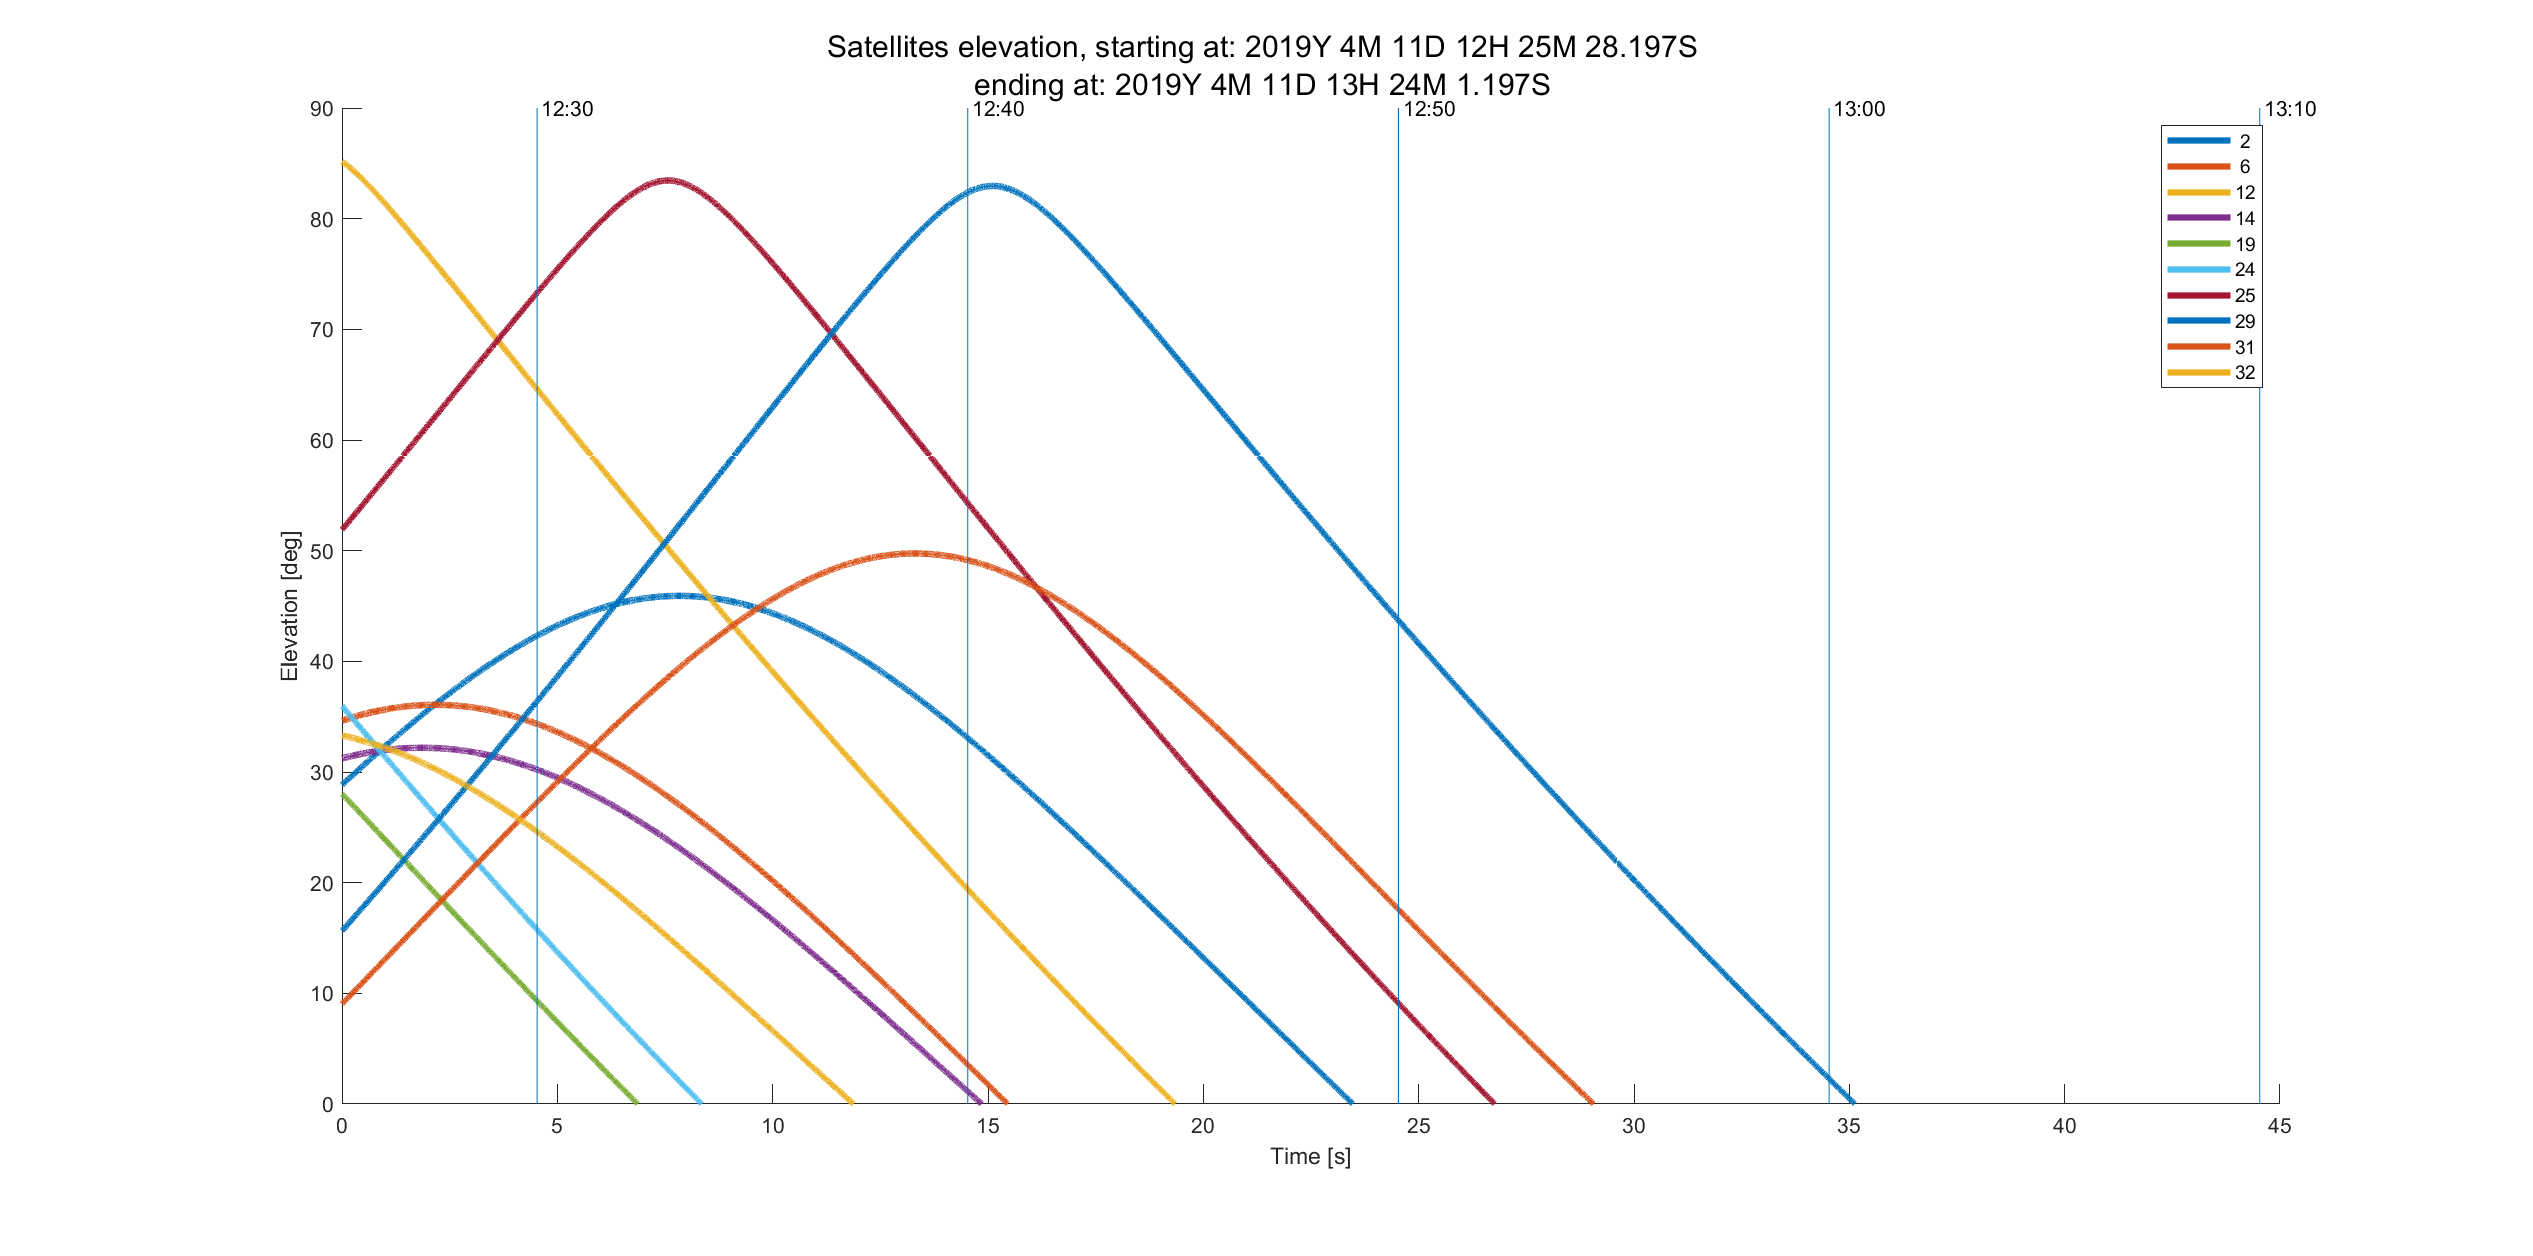
\includegraphics[width=\textwidth]{Results/elev6H.eps}
\caption{\label{fig:el6H} Elevation (upper), Azimuth (middle) Distance (lower) for GPS-satellites with regards to receiver at position 59.353$^o$N, 18.073$^o$E.}
\end{figure}
\begin{figure}
\centering
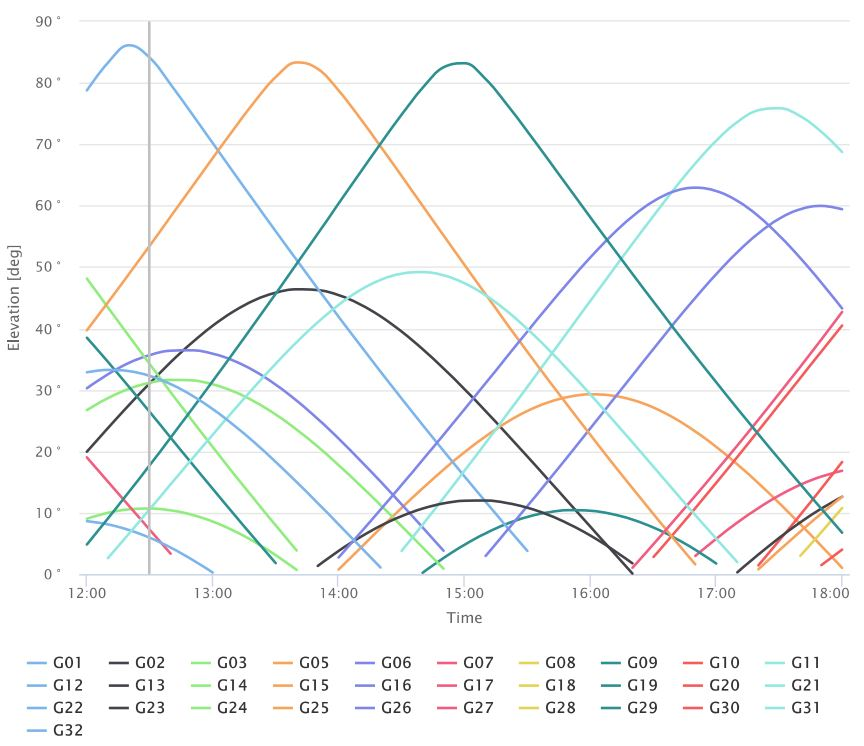
\includegraphics[width=0.7\textwidth]{Results/elevGNSSPlanning.jpg}
\caption{\label{fig:elGNSSPlanning} Elevation plot from \url{gnssplanning.com} at coordinates 59.353$^o$N, 18.073$^o$E. }
\end{figure}

\section{Position estimate using global positioning}
This section presents the results of the onboard estimate and the individual global positioning. Sampling was performed for approximately 30 minutes per receiver in each direction.
\subsection{Position from onboard estimate} \label{onBoardSolution}
The result of the two individual estimates is illustrated in figures \ref{fig:histN}-\ref{fig:histE} from a approximately 8500 samples per receiver.
\begin{figure}
\centering
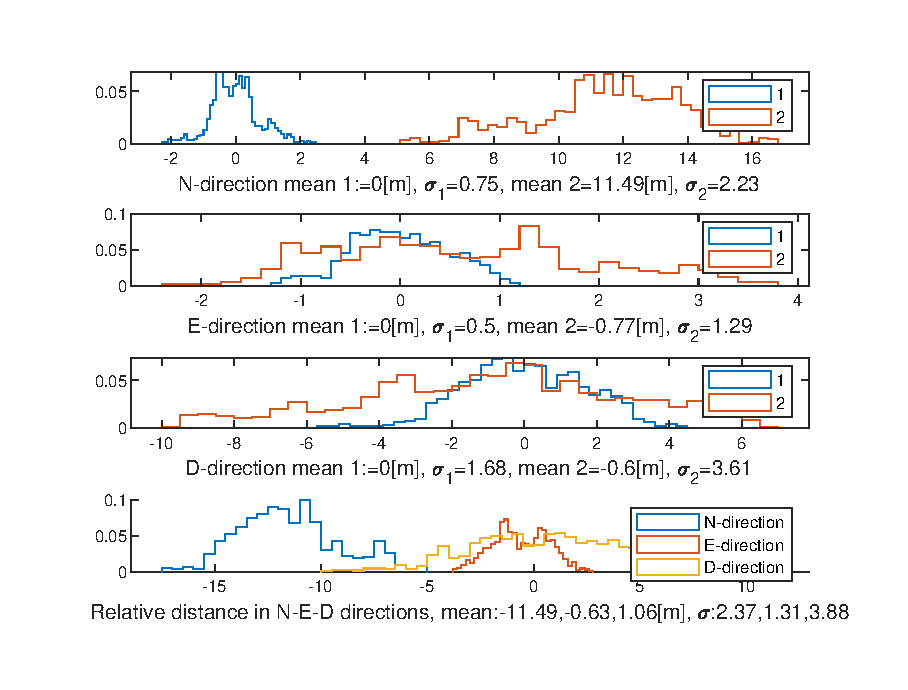
\includegraphics[width=\textwidth]{Results/GPShist10mN.eps}
\caption{\label{fig:histN} Histogram over position over time with an East direction baseline of 10 m separate per direction, N-direction (upper), E-direction (second from top), D-direction (second from bottom), Relative distance for all three directions at synchronised times (bottom)}
\end{figure}
\begin{figure}
\centering
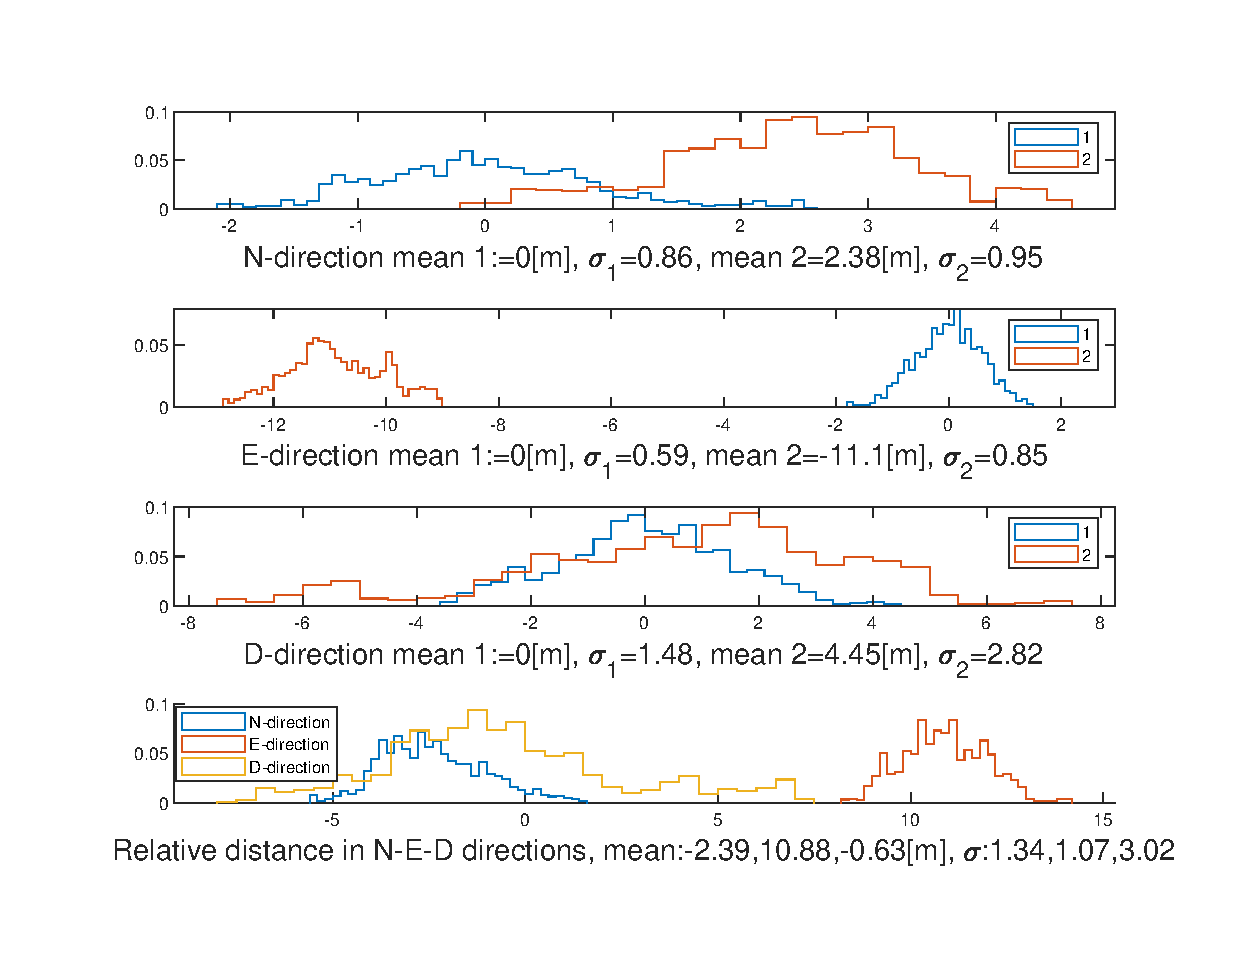
\includegraphics[width=\textwidth]{Results/GPShist10mE.eps}
\caption{\label{fig:histE} Histogram over position over time with an North direction baseline of 10 m separate per direction, N-direction (upper), E-direction (second from top), D-direction (second from bottom), Relative distance for all three directions at synchronised times (bottom)}
\end{figure}
The estimate is transformed from an ECEF frame to a NED frame using the first registered position from receiver 1. Here the origin has been set to the mean over time for receiver 1 per direction. The ideal outcome would be positions separated by 10 m in one direction and 0 in the others and have a Gaussian distribution. 
\par
The standard deviation per direction and observation series is presented in table \ref{table:resultsHistIS}. $\sigma_{12}$ has been introduced to denote the standard deviation in the relative estimate between the receivers. It is apparent from the images and the data in the table that the standard deviation of receiver 2 is greater than that of receiver 1 for all directions in both observations. It can be noted that receiver 2 is that which was placed close to the pin in figure \ref{fig:Uggleviken} and was closer to the forest right north of it than receiver 1 for both observations.
\begin{table}[h!]
  \begin{center}
    \begin{tabular}{|c|c|c|c|}\hline
		& \textbf{North} & \textbf{East}& \textbf{Down}\\
      \hline
      	N-dir \\ \hline
      	$\Delta p$& -11.5 & -0.6 & 1\\ \hline
		$\sigma_1$& 0.8 & 0.5 & 1.7 \\\hline
		$\sigma_2$ & 2.2 & 1.3 & 3.6 \\ \hline
		$\sigma_{12}$& 2.4 & 1.3 & 3.9 \\ \hline
		N-dir\\ \hline
		$\Delta p$& -2.4& 10.9 & -0.6 \\ \hline
		$\sigma_1$& 0.9 & 0.6 & 1.5 \\\hline
		$\sigma_2$ & 1 & 0.9 & 2.8 \\ \hline
		$\sigma_{12}$ & 1.3 & 1 & 3 \\ \hline
    \end{tabular}
    \caption{\label{table:resultsHistIS} Mean and standard deviation of position from on board individual estimate, as well as the relative estimate. Values referring to the figures \ref{fig:histN}-\ref{fig:histE}}
  \end{center}
\end{table}

\subsection{Least square estimator from raw observation data}\label{leastSquareEstimator}
The global position for two receivers is also calculated as described in section \ref{stateEst} using the transmitted ephemeris data to calculate the satellite positions in ECEF coordinates in combination with raw observational data. The observations are weighted using their respective SNR-value as described in equation (\ref{SNRWeights}).
The results are based on approximately 8500 samples per receiver and observation series. They are presented in two ways:
\begin{itemize}
\item The positions are calculated independently for the receivers, using all available satellites.
\item Only satellites which are shared between receivers are used.
\end{itemize}
When fully independent estimates are used, several satellites may go in and out of tracking between two epochs, leading to a change in position estimate due to e.g. error in satellite position estimate. The result of fully independent estimates are presented in figures \ref{fig:globalPosAllSV}. The mean and variance, per direction for the two observations are presented in table \ref{table:resultsPosAllSat}.
\begin{figure}[H]
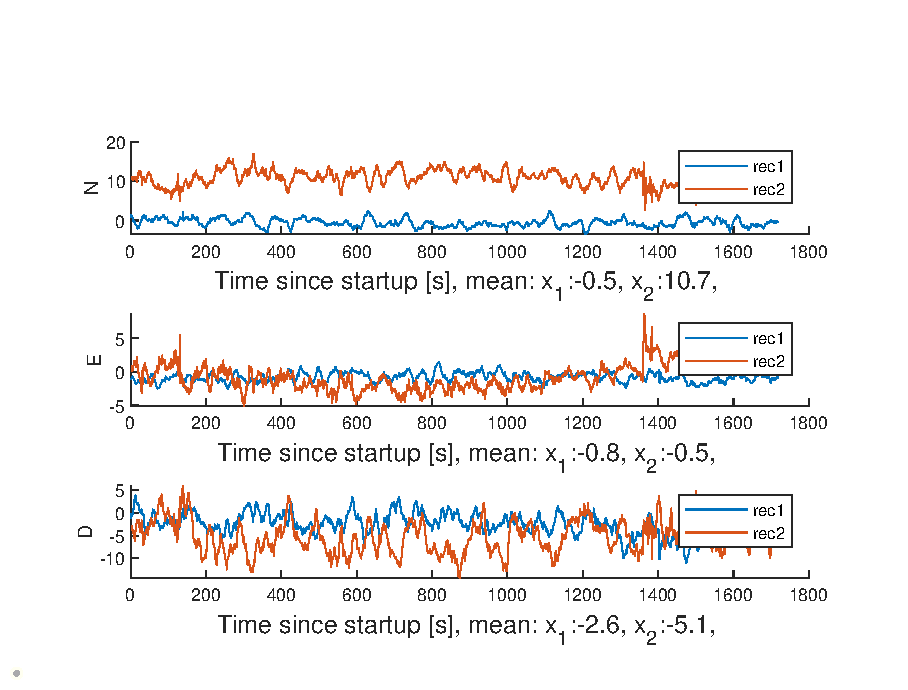
\includegraphics[width=1\textwidth]{Results/DistNED30MinNAllSat}
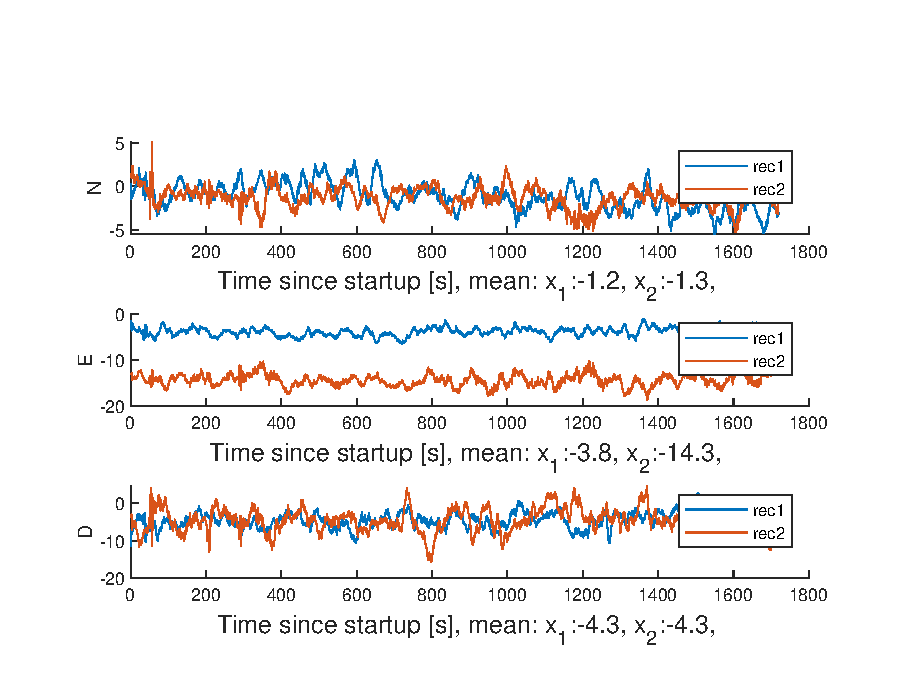
\includegraphics[width=1\textwidth]{Results/DistNED30MinEAllSat}
\caption{\label{fig:globalPosAllSV} Independent global position estimates for two receivers separated 10m N-direction (upper) and E-direction (lower) in N, E and D directions respectively, where the origin is set to true position. All satellite information known to respective receiver is used.}
\end{figure}
\begin{table}[h!]
\begin{minipage}{0.45\linewidth}
  \begin{center} 
    \begin{tabular}{|c|c|c|c|}\hline
		& \textbf{North} & \textbf{East}& \textbf{Down}\\
      \hline
      	E-dir \\ \hline
      	$\Delta p$& 10.2 & 0.3 & -2.6\\ \hline
		$\sigma_1$& 1.6 & 0.9 & 2.2 \\\hline
		$\sigma_2$ & 1.2 &1.3 & 3.3 \\ \hline
		N-dir\\ \hline
		$\Delta p$& -0.1& -10.5 & 0 \\ \hline
		$\sigma_1$& 1 & 0.7 & 2.4 \\\hline
		$\sigma_2$ & 2 &2.1 & 3.5 \\
		\hline
	\end{tabular}
    \caption{\label{table:resultsPosAllSat} Averaged values of difference in position and standard deviation of  position estimate per direction, receivers use all available information. Values referring to measurements in figure \ref{fig:globalPosAllSV}}
  \end{center}
  
\end{minipage}
\begin{minipage}{0.45\linewidth}
  \begin{center}
    \begin{tabular}{|c|c|c|c|}\hline
		& \textbf{North} & \textbf{East}& \textbf{Down}\\
      \hline
      	E-dir\\ \hline
      	$\Delta p$& 10.6& 0.6 & -1 \\ \hline 
		$\sigma_1$& 1.8 & 1.4 & 2.5 \\\hline
		$\sigma_2$ & 1.4 &1.3 & 3.8 \\ \hline
		N-dir\\ \hline
		$\Delta p$ & -1.4 & -11.9 & -0.4 \\ \hline
		$\sigma_1$& 1 & 0.7 & 2.5 \\\hline
		$\sigma_2$ & 2 &2.1 & 3.5 \\
		\hline
    \end{tabular}
    \caption{\label{table:resultsPosSharedSat} Averaged values of difference in position and standard deviation of  position estimate per direction when only shared satellites are used. Values referring to measurements in figure \ref{fig:globalPosSelectSV}}
  \end{center}
\end{minipage}
\end{table}
As a comparison, the position estimate for when only satellites shared  between receivers is presented in figure \ref{fig:globalPosSelectSV}. This is done by extracting only those satellites which are observed by both receivers from the logged data. The mean and variance per direction for the two observations is presented in table \ref{table:resultsPosSharedSat}. The results are very similar but slightly worse for the solution where only shared satellites are used. This leads to the conclusion that this seems to have no positive effect.

\begin{figure}[H]
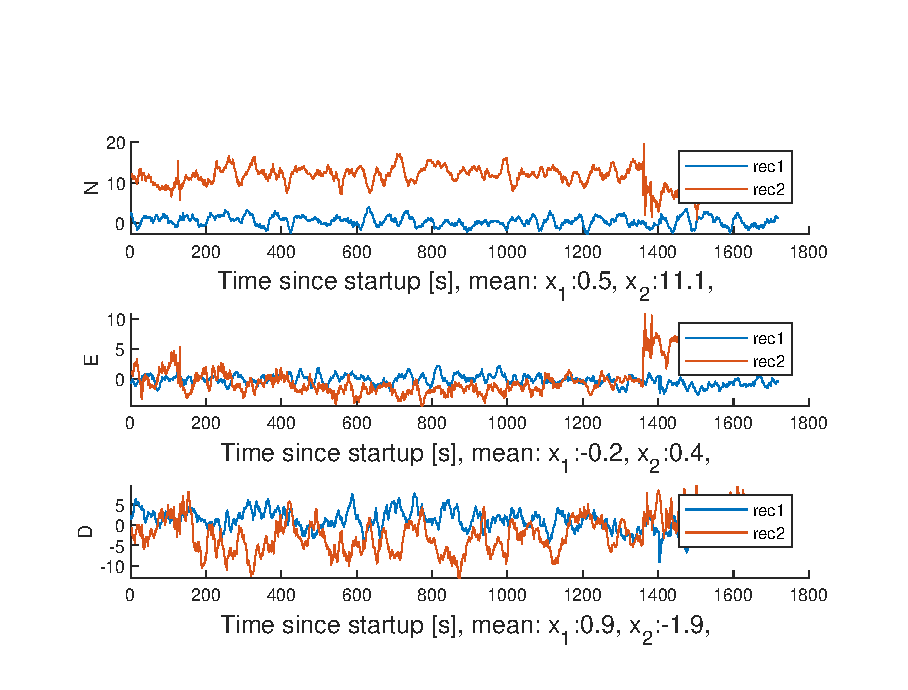
\includegraphics[width=1\textwidth]{Results/DistNED30MinNSharedSat}
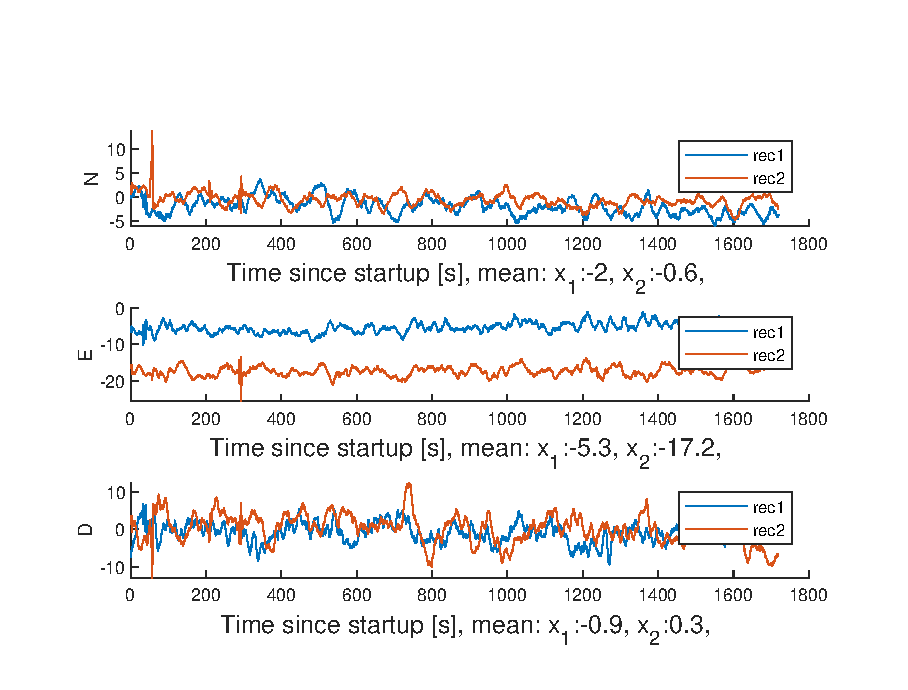
\includegraphics[width=1\textwidth]{Results/DistNED30MinESharedSats}
\caption{\label{fig:globalPosSelectSV} Independent global position estimates for two receivers separated 10m N-direction (upper) and E-direction (lower), origin is set to true position. Only satellite data shared between receivers is used.}
\end{figure}
\section{Relative estimates}
\subsection{Histograms of relative position and noise estimates}\label{histogramDD}
The same sampling process as above is used, using only the momentary estimate from pseudorange measurements, is shown in figures (\ref{fig:histRel1hN}-\ref{fig:histRel1hE}). The mean and standard deviation for each direction of the two sample periods is presented in table \ref{table:resultsRel}.
\begin{figure}[H]
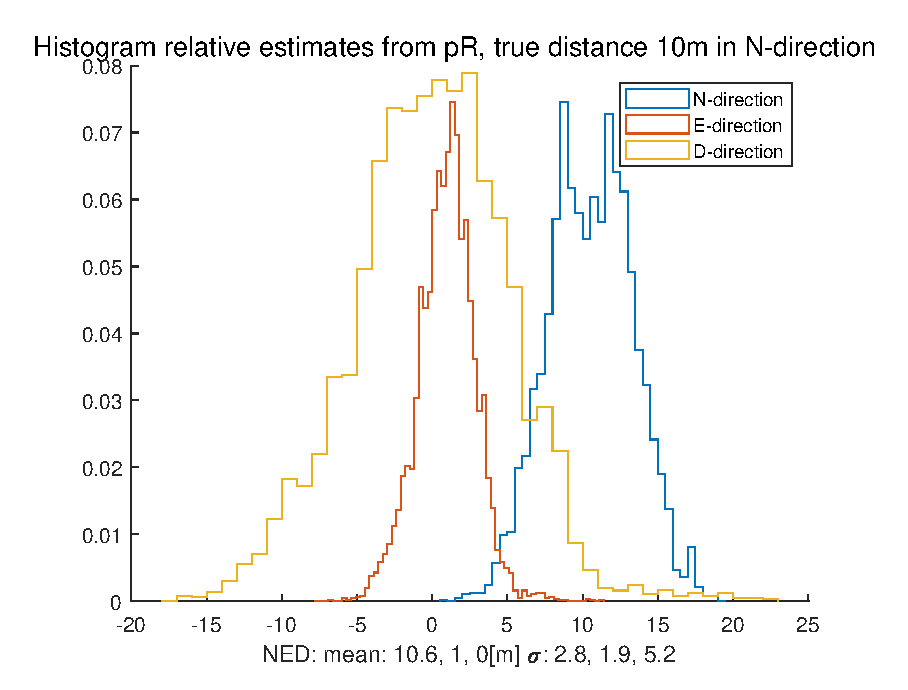
\includegraphics[width=\textwidth]{Results/histRel30MinN}
\caption{\label{fig:histRel1hN}}
%\caption{\label{fig:histRel1hN} Position over time with a North direction baseline of 10 m}
\end{figure}
\begin{figure}
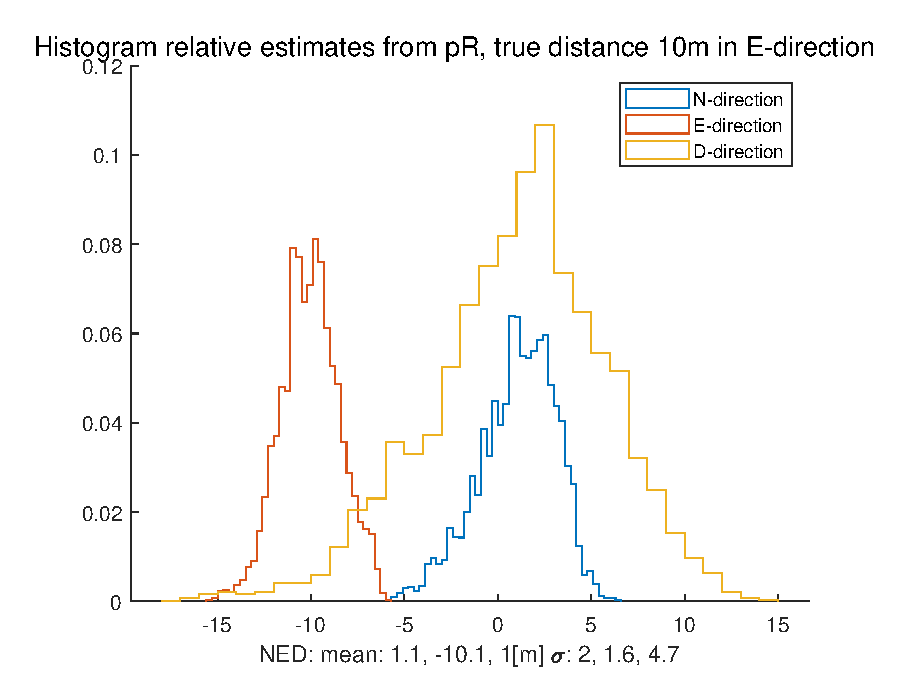
\includegraphics[width=\textwidth]{Results/histRel30MinE}
\caption{\label{fig:histRel1hE}}
%\caption{\label{fig:histRel1hE} Position over time with an East direction baseline of 10 m}
\end{figure}

\begin{table}[!htb]
  \begin{center}
    \begin{tabular}{|c|c|c|c|}\hline
		& \textbf{North} & \textbf{East}& \textbf{Down}\\
      \hline
      True[m]& 10 & 0&0\\ \hline
      Mean[m] &11.4 & 0.1 & -0,5\\ \hline
		$\sigma$& 4.3 & 2.9 & 7.7 \\\hline
		True[m] & 0 &10&0\\ \hline
		Mean[m] & 2 & -11.4 & 0.7\\ \hline
		$\sigma$ & 2.3 &1.8 & 4.7 \\
		\hline
    \end{tabular}
    \caption{\label{table:resultsRel} Averaged values of difference in position and standard deviation of position estimate per direction for a DD-estimate. Values referring to measurements in figure (\ref{fig:histRel1hN}-\ref{fig:histRel1hE})}
  \end{center}
\end{table}
The results from section \ref{onBoardSolution} is compared those presented in figures (\ref{fig:histRel1hN}-\ref{fig:histRel1hE}) in figures  (\ref{fig:DDandInternalN}-\ref{fig:DDandInternalE}). The plots clearly show that the standard deviation of the DD-estimate at best is equal to, or close to equal to that of the onboard solution but generally can be expected to be greater.
\begin{figure}[!htb]
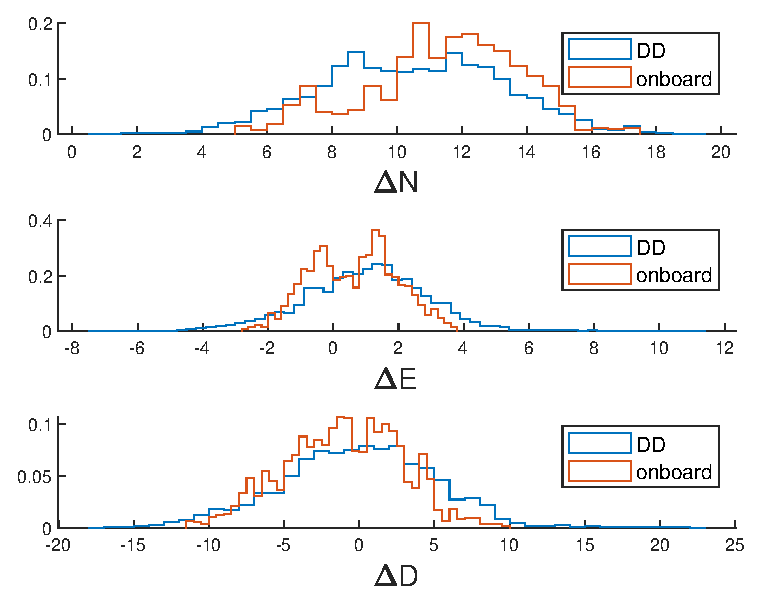
\includegraphics[width=\textwidth]{Results/Nhist.eps}
\caption{\label{fig:DDandInternalN} Histogram over difference in position over time with a North direction baseline of 10 m. Plots showing results of DD and onboard solution.}
\end{figure}
\begin{figure}[!htb]
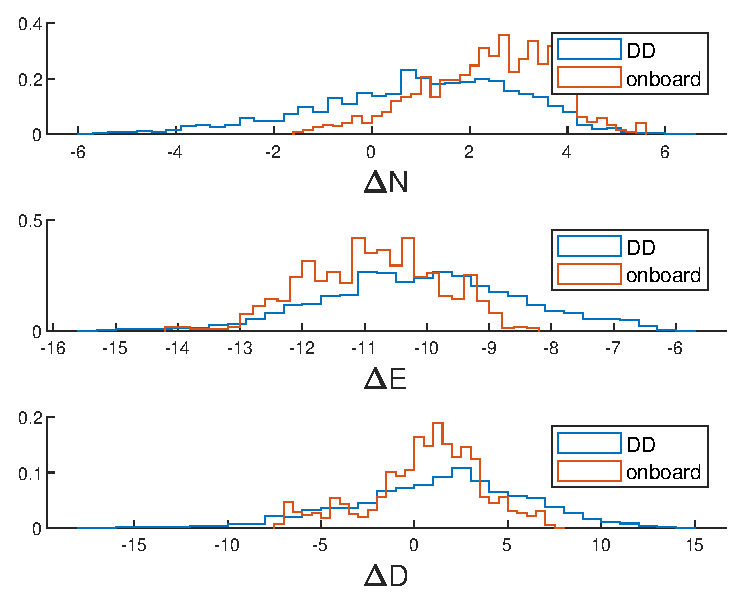
\includegraphics[width=\textwidth]{Results/Ehist.eps}
\caption{\label{fig:DDandInternalE} Histogram over difference in position over time with an East direction baseline of 10 m. Plots showing results of DD and onboard solution.}
\end{figure}

\section{RMSE of relative position from global positioning and DD estimate }\label{RMSEsection}
All the simulations described in section \ref{RMSE} are performed using a Gaussian white noise level of 1 m. The positions are then calculated first using two independent global fixes, and then the DD relative position, for increasing magnitude of the bias. In figures (\ref{fig:Nsim1}-\ref{fig:Nsim20}) the simulated results are shown of increasing the magnitude of the bias which is set to respectively 1, 10 and 20 m. It's apparent that for the global positioning the error grows with the bias, while the differenced position appears to be unchanged which motivates the use of this method for high levels of the common noise $\nu$ shared between the receivers.
\begin{figure}[!htb]
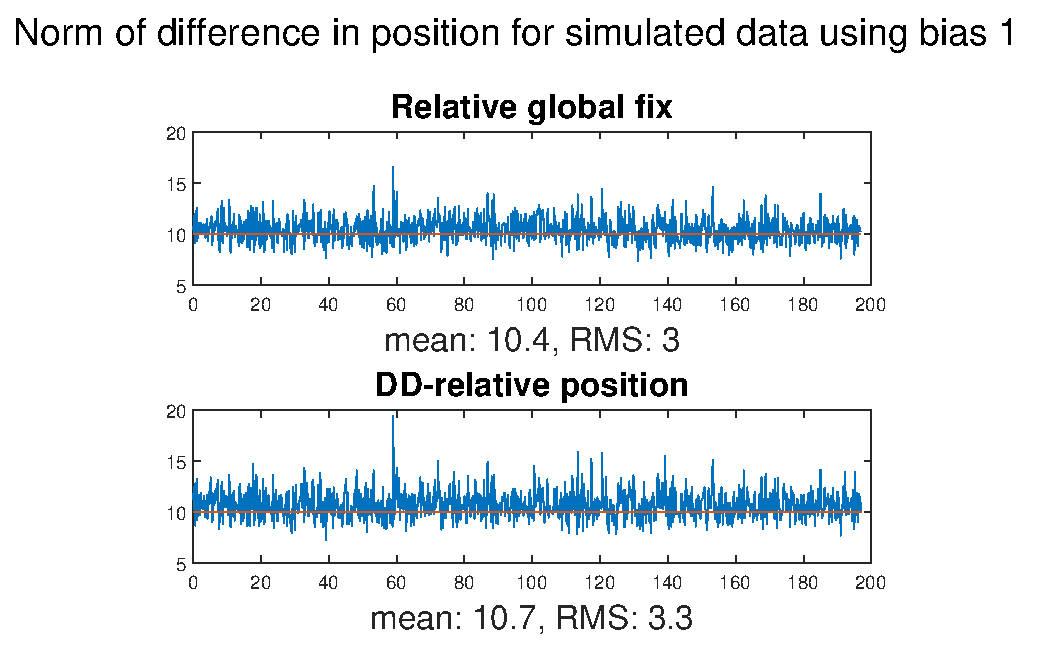
\includegraphics[width=\textwidth]{Results/MSEplots/Nsim1.eps}
\caption{\label{fig:Nsim1}}
%\caption{\label{fig:Nsim2} Result of relative position from global position fixes (upper) and DD relative position (lower) using simulated data with a magnitude of 1 for the bias.}
\end{figure}
\begin{figure}[!htb]
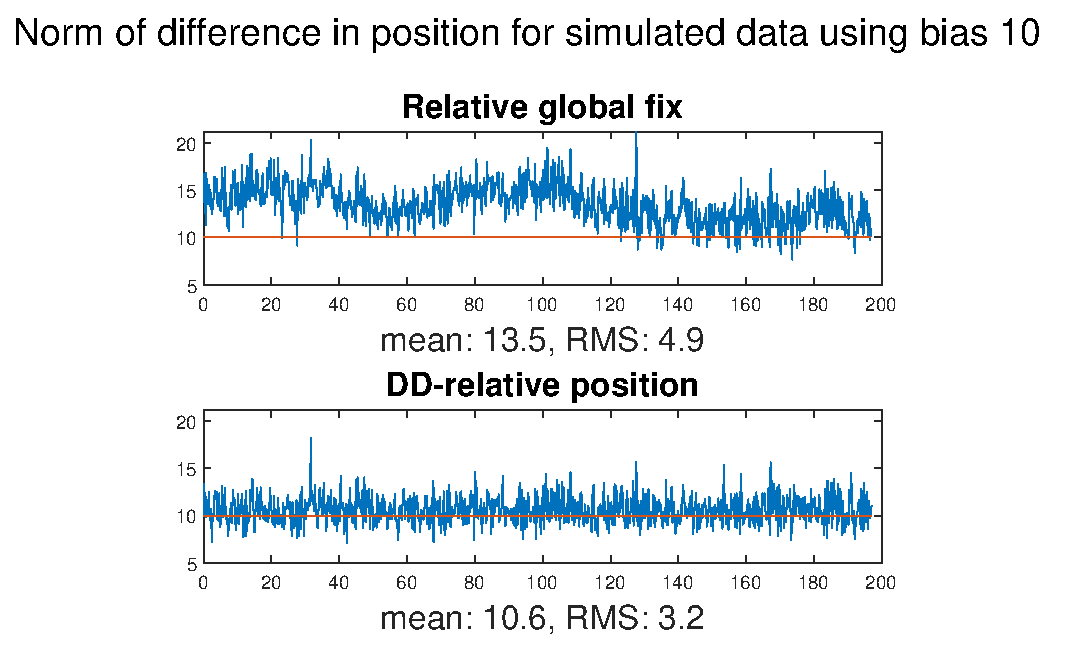
\includegraphics[width=\textwidth]{Results/MSEplots/Nsim10.eps}
\caption{\label{fig:Nsim10}}
%\caption{\label{fig:Nsim10} Result of relative position from global position fixes (upper) and DD relative position (lower) using simulated data with a magnitude of 10 for the bias.}
\end{figure}
\begin{figure}[!htb]
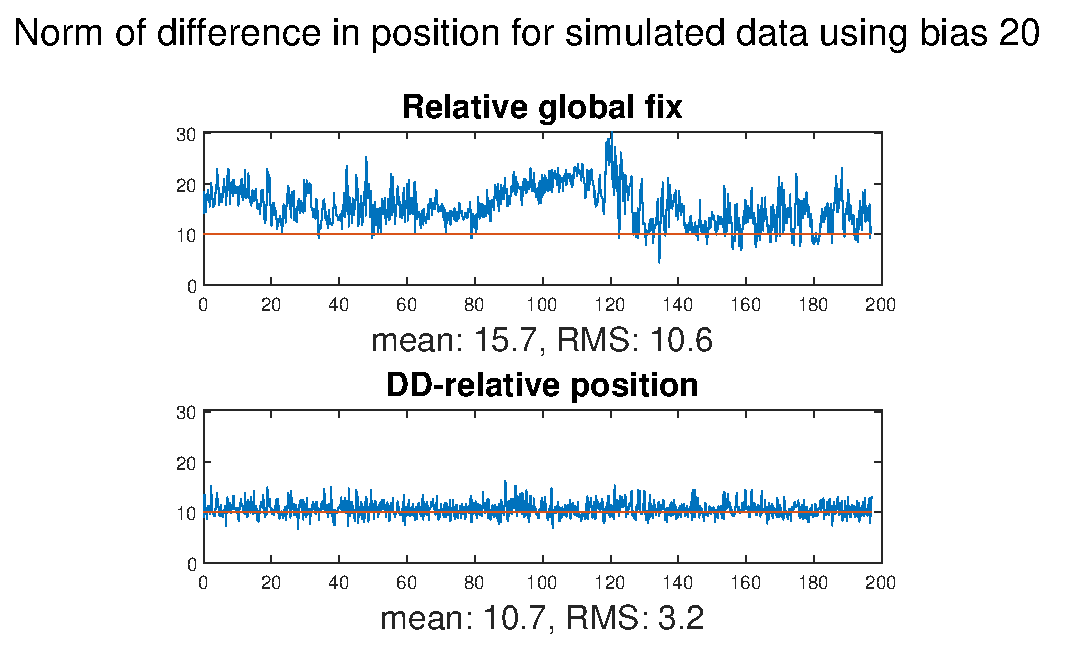
\includegraphics[width=\textwidth]{Results/MSEplots/Nsim20.eps}
\caption{\label{fig:Nsim20}}
%\caption{\label{fig:Nsim20} Result of relative position from global position fixes (upper) and DD relative position (lower) using simulated data with a magnitude of 20 for the bias.}
\end{figure}
\par
The result of the same calculations performed for the actual observation data is presented in figures (\ref{fig:Nobs}-\ref{fig:Eobs}) with a 10 m separation in north and east direction separation respectively. The calculaed RMSE values are, respectively in the north and east direction for the global estimate and DD solutions are 5.6 and 4.9 m in north direction, and 5 and 4.8 for east-direction. The DD-method thus performs slightly better for that of the DD-relative position in both cases.
\begin{figure}[!htb]
\centering
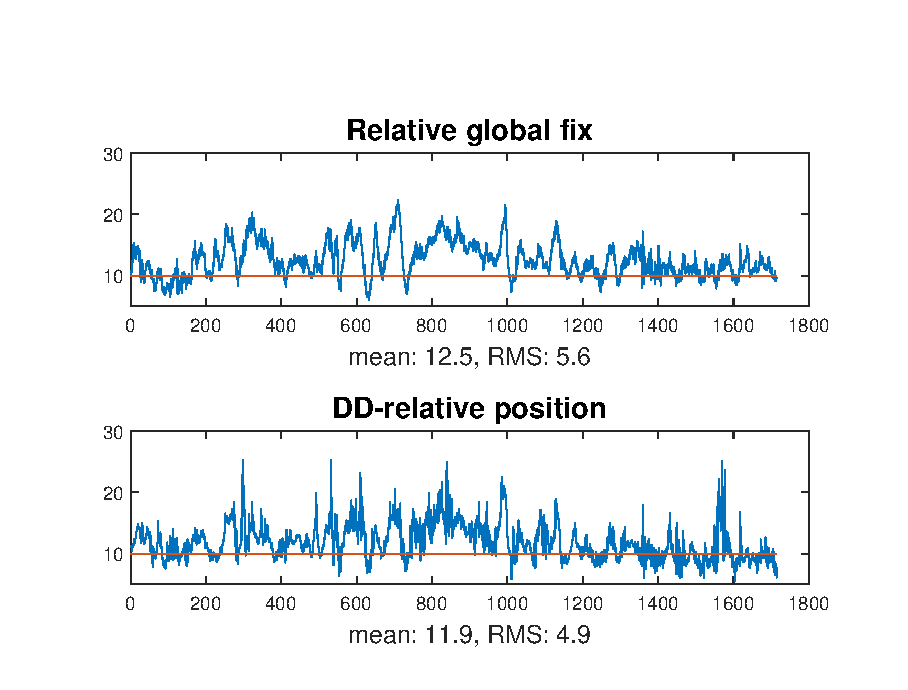
\includegraphics[width=\textwidth]{Results/MSEplots/Nobs.eps}
\caption{\label{fig:Nobs} Result of relative position from global position fixes (upper) and DD relative position (lower) from observation data in a north-direction separation.}
\end{figure}
\begin{figure}[!htb]
\centering
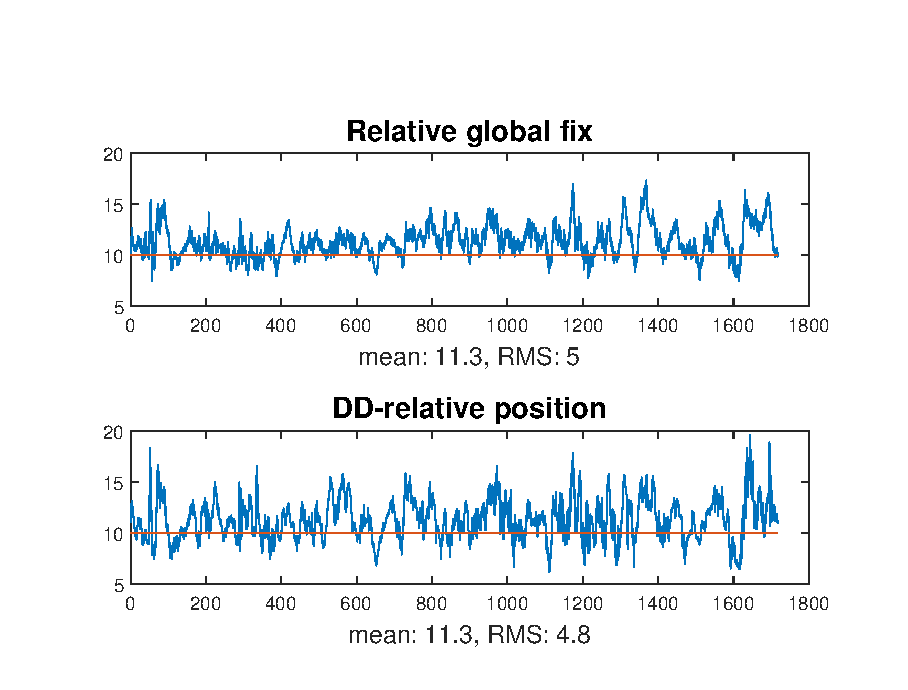
\includegraphics[width=\textwidth]{Results/MSEplots/Eobs.eps}
\caption{\label{fig:Eobs} Result of relative position from global position fixes (upper) and DD relative position (lower) from observation data in an east-direction separation.}
\end{figure}

\section{DOP values}\label{sectionDOP}
The DOP-values of the observations series are calculated as presented in section \ref{satelliteGeometry}. If the DOP values are poor, then the performance of the estimator can also be expected to be poor. A notable difference between the results of the global estimates and the DD estimate is that the TDOP-value isn't included in the equations for the latter as the receiver bias $\Delta t_{rec}$ isn't estimated. This results in the DOP-matrix being reduced to a $3\times3$ matrix. Besides that, calculations are performed equal to a global estimate DOP-value.

\begin{comment}
In order to evaluate the variance of the estimates, the results of the observations are tied to their respective DOP-values, calculated as described in equations \ref{eq:HDOP} and \ref{eq:VDOP}. An estimate of the UERE values can be calculated from equation \ref{UERE} as 
\begin{align}\label{epsilon}
\epsilon=\frac{\sigma}{q}
\end{align}
The value of $\epsilon$ will be presented as $\epsilon_H$ and $\epsilon_V$, where $\epsilon_H$ is the root sum squared of the $\sigma_N$ and $\sigma_E$ values.
\end{comment}
\subsection{DOP values global estimates} 
In figure \ref{fig:DOP1}-\ref{fig:DOP2}, the DOP values are presented. The values are quite similar for receiver 1 and receiver 2. With a small baseline distance, only the satellites observed should produce a difference in their DOP values. The HDOP and VDOP value with a mean of around 0.5 and 2 respectively at N-separation observation, and mean of around 0.45 and 1.6 for the E-separation observation. These are all well within the acceptable range of what can be considered good geometry, as presented in section \ref{satelliteGeometry}.
\begin{comment}
Using the information from table \ref{table:resultsPosAllSat}, 
and the relation in equation \ref{epsilon} gives an estimate of the noise level. 
The $\epsilon_H$ and $\epsilon_H$ values are calculated per receiver
\\For the N-direction sample series:
\begin{align*}
\epsilon_{H,1}&=2.4 & \epsilon_{H,2}=5.8\\
\epsilon_{V,1}&=1.2 & \epsilon_{V,2}=1.8
\end{align*}
For the E-direction sample series: 
\begin{align*}
\epsilon_{H,1}&=4.1 & \epsilon_{H,2}=3.9\\
\epsilon_{V,1}&=1.4 & \epsilon_{V,2}=2.0
\end{align*}
\end{comment}
\begin{comment}
ALSSAT
N-DIR
sigma1 1N 0.7E ==> 1.2, 2.4D, eps=1.2/0.5H, 2.4/2=1.2V
sigma2 2N 2.1E==>2.9, 3.5D, eps=2.9/0.5=5.8, 3.5/2=1.8V
E-DIR
sigma1 1.6N, 0.9E ==> 1.8,  2.2D ger att eps=1.8/0.45=4.1H, 1.38V
sigma2 1.2 1.3 ==1.7 3.3D eps= 1.7/0.45=3.9, 3.3/1.6=2.01V

SHAREDSAT
DOP VALUES E:
H: 1.1, V: 4.24
DOP VALUES N:
H: 1.1, V: 3.2
E
sigma1: 1.8N, 1.4E ==> 2.28, 2.5D ger eps=2.28/1.1=2.01, 2.5/4.24=0.5
sigma2: 1.4N, 1.3E ==> 1.91, 3.8D ger eps=1.91/1.1=1.73, 3.8/4.24=0.89
N
sigma1: 1N, 0.7E ==>  1.22, 2.5D ger 1.22/1.1=1.11, 2.5/3.2=0.78
sigma2: 2N, 0.7E ==> 2.12, 3.5D ger 2.12/1.1=1.92, 3.5/3.2=1.09


\end{comment}
\begin{figure}[!htb]
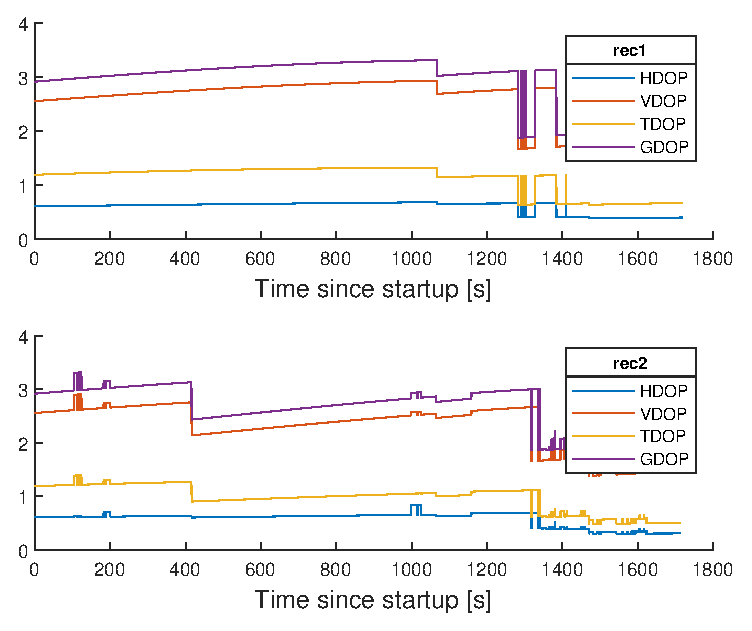
\includegraphics[width=\textwidth]{Results/DOP_N}
\caption{\label{fig:DOP1} Individual DOP values for two receivers separated 10m in N-direction, upper receiver 1, lower receiver 2.}
\end{figure}
\begin{figure}[!htb]
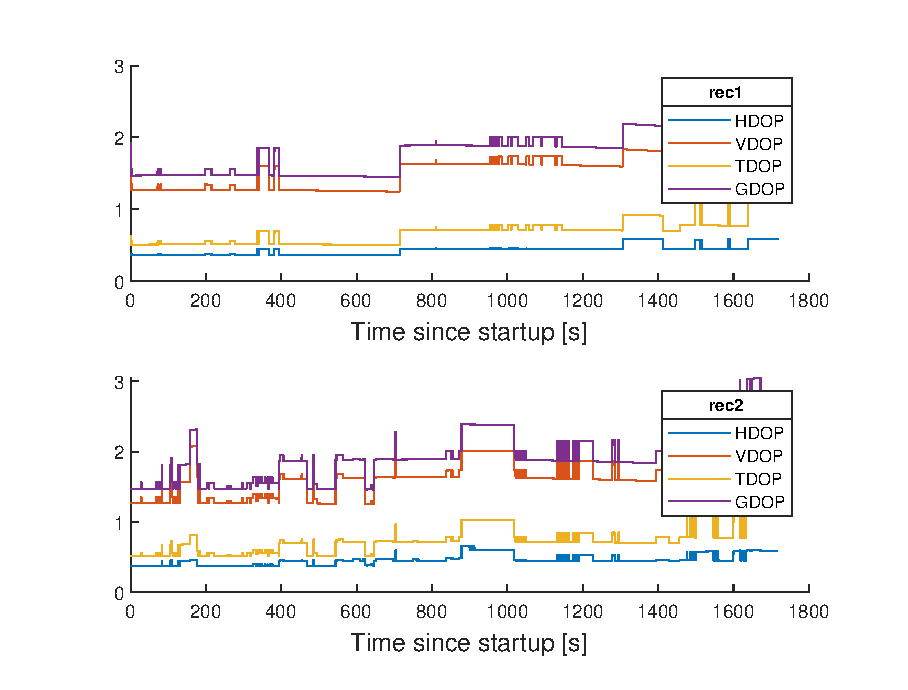
\includegraphics[width=\textwidth]{Results/DOP_E}
\caption{\label{fig:DOP2} Individual DOP values for two receivers separated 10m in E-direction, upper receiver 1, lower receiver 2.}
\end{figure}

\subsection{Double differenced DOP values}
In figures \ref{fig:DD_DOP1}-\ref{fig:DD_DOP2} the HDOP and VDOP values are calculated as previously mentioned, but only the directional matrix given by \ref{eq:DD-LS} is used as the clock errors aren't estimated, which only produces an estimate of the geometric uncertainty. The values have a mean at 0.56 for the HDOP and 0.77 for VDOP in the N-direction separated observation, and 0.46 and 0.57 for the E-separated observation. 
\begin{figure}[!htb]
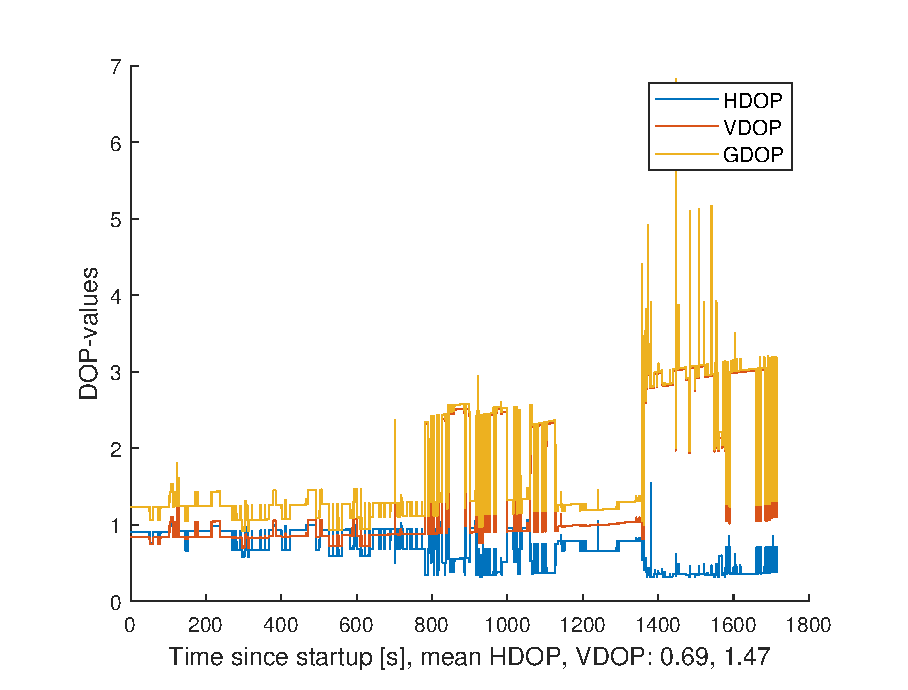
\includegraphics[width=0.8\textwidth]{Results/DDDOPN}
\caption{\label{fig:DD_DOP1} DOP values from DD-estimate for two receivers separated 10m in N-direction.}
\end{figure}
\begin{figure}[!htb]
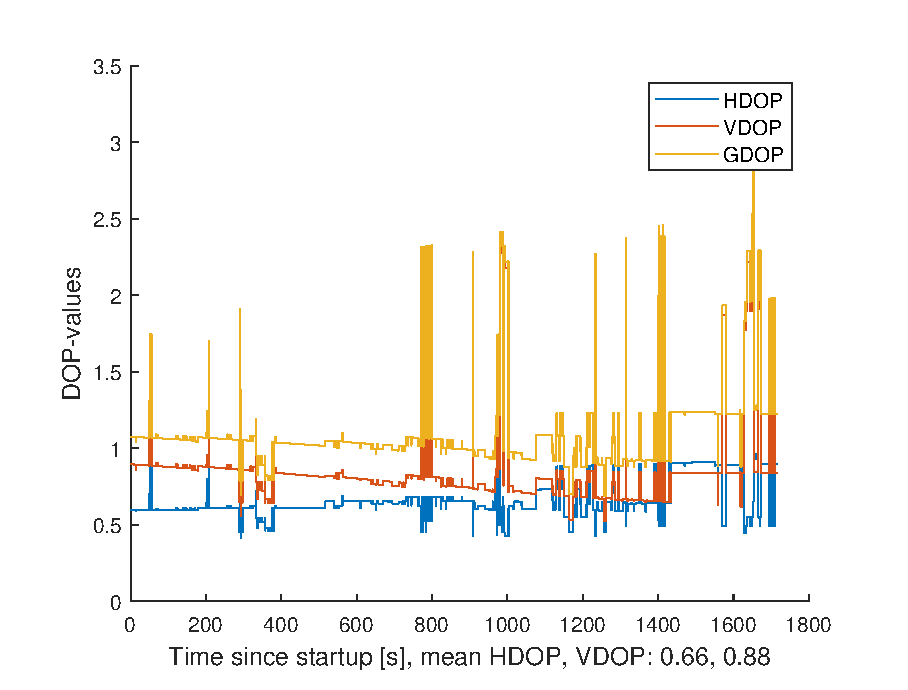
\includegraphics[width=0.8\textwidth]{Results/DDDOPE}
\caption{\label{fig:DD_DOP2} DOP values DD-estimate for two receivers separated 10m in E-direction.}
\end{figure}
The GDOP value, calculated as $$q_G=\sqrt{q^2_H+q^2_V}$$ when the TDOP value is omitted also indicate a very good geometry with the exception of a few samples where it exceeds 3. 
\begin{comment}
Using the values from \ref{table:resultsRel} and equation \ref{epsilon} gives that the calculated values of $\epsilon_H$ is, for the north and east observation respectively equal to 9.26 and 6.35, and $\epsilon_V$ is 10 and 10.2. 

DOP N
H 0.56 V 0.77
DOP E
H 0.46 V 0.57
SIGMA N: 4.3N, 2.9E, 7.7D
SIGMA E: 2.3N, 1.8E, 4.7D
eps_H=9.26 and 6.35
eps_V=10 and 10
\end{comment}


\end{document}
